%----------------------------------------------------------------------------
\chapter{Design and implementation}
\label{chap:designimplementation}
%----------------------------------------------------------------------------

Task flow again: simulation and extraction, detector, webviz


\section{Choosing the sensor suite}

Mounting cameras around the vehicle to have an all around vision is an essential
design strategy, as we have seen in the work of other companies in
\autoref{chap:relatedwork}. However we will need to determine depth as well. I
decided to use only cameras in a stereoscopic structure to create 4 stereo sides
around the vehicle. The following model shows the design setting \refstruc{fig:3dmodel3}.

\begin{figure}[!ht]
    \centering
    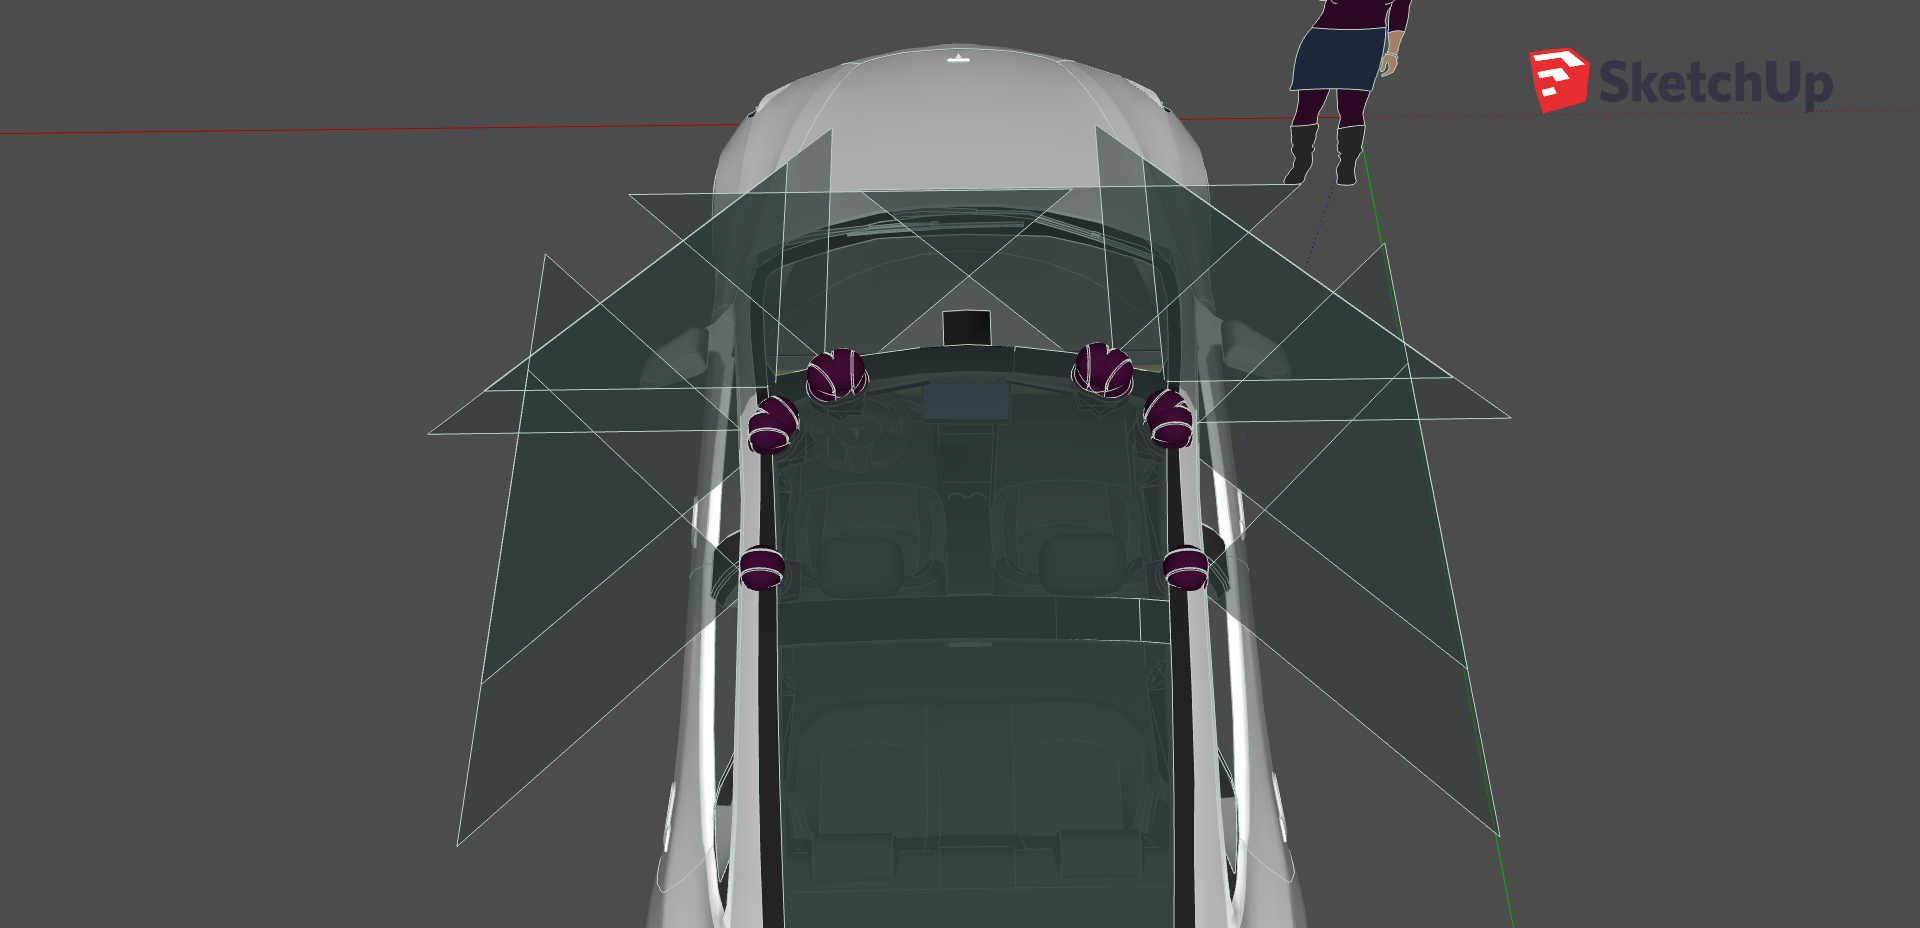
\includegraphics[width=150mm, keepaspectratio]{figures/3dmodel3.png}
    \caption{The stereo camera setting I used on top of the virtual Tesla Model 3}
    \label{fig:3dmodel3}
\end{figure}

The setting is the following: 
\begin{itemize}
    \item Variations in viewpoint
    \item Difference in illumination
    \item Hidden parts of images, occulsion
    \item Background Clutter
\end{itemize}

\section{Tools used}
- Linux Ubuntu
- VS Code
- Python, Scripts, Conda, Jupyter

\section{Carla simulator}

CARLA\cite{Dosovitskiy17} is an open-source simulator for autonomous driving
research. It is written in C++ and provides a very accessible Python API to
control a lot of the simulaton execution. CARLA has been developed from the
ground up to support development, training, and validation of autonomous driving
systems. In addition to open-source code and protocols, CARLA provides open
digital assets (urban layouts, buildings, vehicles) that were created for this
purpose and can be used freely. The simulation platform supports flexible
specification of sensor suites, environmental conditions, full control of all
static and dynamic actors, maps generation and much more. It is developed by the
Barcelonian university UAB's computer vision CVC Lab supported by Intel, Toyota,
GM and others. The repository for the project is at \url{https://github.com/carla-simulator}

It provides Scalability via a server multi-client architecture: multiple clients
in the same or in different nodes can control different actors. CARLA exposes a
powerful API that allows users to control all aspects related to the simulation,
including traffic generation, pedestrian behaviors, weathers, sensors, and much
more. Users can configure diverse sensor suites including LIDARs, multiple
cameras, depth sensors and GPS among others. Users can easily create their own
maps following the OpenDrive standard via tools like RoadRunner. CARLA provides
integration with ROS via their ROS-bridge

I used CARLA 9.8.0 in the project that was the latest at the time (2020 March
09). Carla has a primary support for Linux so I could run it easly on Ubuntu. It
requires a decent GPU otherwise the simulation is going to be slow.


\section{Configuring the simulation}
- Recorder
- Stereo imaging
- Coordinate system
- Simulation imaging: HD 720p, Camera matrix, compression, noise, reality,
distortion, focus, etc, cropping, occlusion, etc, throughoutput
\section{Extracted data}
- Rendering file structure 
- Extracted data - section
- Coordinate system
\section{Detector}
    \subsection{OpenCV}
    \subsection{Detectron}
    - Pretrained models
    - Comparison
    - Object detection and localization
    - Instance segmentation
    \subsection{Depth estimation}
    \subsection{Back projection}
        Camera setting
    - Inverse transformation explain, Translation: same matrix as camera why
    - Stereo Block Matching Algorithm (newer)
    \subsection{Pseudo-code}
        Final pseudo code
\section{Web visualizer}
        Web visualizer
    -  Framework
    -  Usage and results